\documentclass{article}
\usepackage{float}
\usepackage[most]{tcolorbox}
\usepackage[a4paper, top=4cm]{geometry}


\title{\textbf{TP DATA832 - Machine Learning} \\Clustering de pays selon le niveau d'aide nécessaire}
\author{Louna CAMAS \& Mathieu DOCHER}
\date{}

\begin{document}

\maketitle

\vspace{3cm}
\tableofcontents

\newpage
\newgeometry{top=3cm, bottom=3cm}
\section{Présentation du dataset}

\noindent Le dataset utilisé contient de nombreuses informations sur différents pays, notamment sur leur situation économique. Pour chaque pays, on dispose du nom du pays et de 9 features quantitatives :

\begin{itemize}
    \item \texttt{country} : le nom du pays
    \item \texttt{child\_mort} : le taux de mortalité des enfants de moins de 5 ans (pour 1000 naissances)
    \item \texttt{exports} : le taux d'exportations de biens et services (en \% du PIB)
    \item \texttt{health} : le taux de dépenses de santé (en \% du PIB)
    \item \texttt{imports} : le taux d'importations de biens et services (en \% du PIB)
    \item \texttt{income} : le revenu net moyen par personne
    \item \texttt{inflation} : le taux d'inflation annuel (en \% du PIB)
    \item \texttt{life\_expec} : l'espérance de vie à la naissance
    \item \texttt{total\_fer} : le nombre moyen d'enfants par femme
    \item \texttt{gdpp} : le PIB par habitant
\end{itemize}
Les données sont assez complètes, même s'il manque plusieurs pays (ex: Mexique) et que certains noms ne sont pas aux normes. Nous avons donc dû réaliser un nettoyage des données que l'on pouvait nettoyer (ex : $\text{United states} \rightarrow  \text{ United States of America}$).

\newpage
\section{Choix de features}

\noindent Pour déterminer quelles features sont les plus utiles, nous avons essayé plusieurs méthodes. \\ \\
La première chose que nous avons tenté de faire est d'afficher la matrice de corrélations entre chaque variable, afin de ne plus prendre en compte les variables qui sont très corrélées, car elles transportent une information similaire (\ref{fig:corr_matrix}). Le résultat ne nous a pas permis de déterminer réellement les variables les plus importantes mais on a pu voir quelques liens (ex: l'espérance de vie et la fertilité).

\begin{figure}[H]
    \centering
    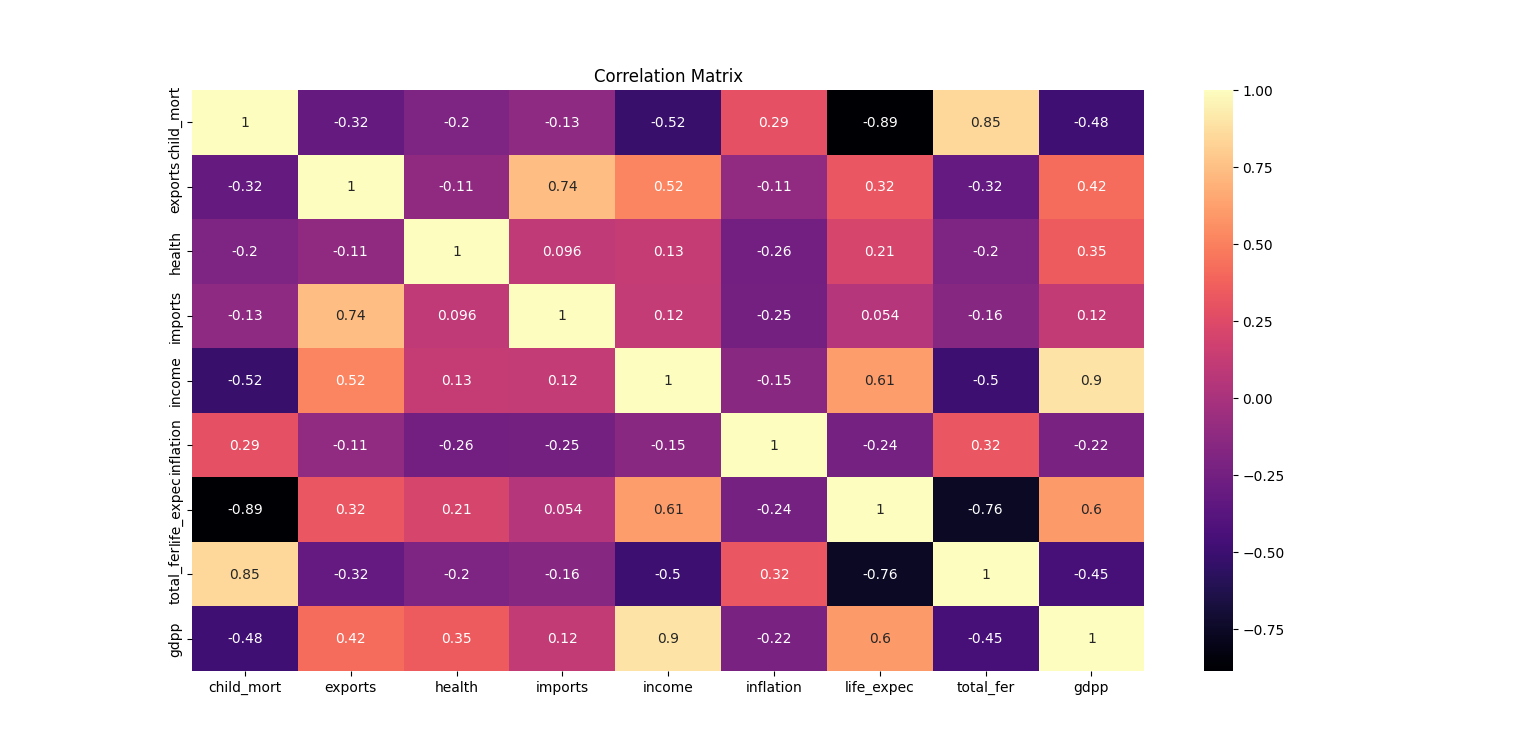
\includegraphics[width=\linewidth]{plot/corr_matrix.png}
    \caption{Matrice de corrélation}
    \label{fig:corr_matrix}
\end{figure}

\noindent Nous avons ensuite essayé d'afficher des histogrammes pour voir les 10 valeurs supérieures (ou inférieures) de certaines variables spécifiques. Ces histogrammes n'aident pas beaucoup pour déterminer les meilleures features à utiliser mais ils permettent de voir s'il y a des redondances dans les pays (ex: les pays avec un taux de mortalité infantile élevé ont souvent un faible PIB par habitant). Voici des exemples de features très corrélées, on voit qu’en général ce sont les mêmes pays :

\begin{figure}[H]
    \centering
    % Première ligne
    \begin{minipage}{0.8\textwidth}
        \centering
        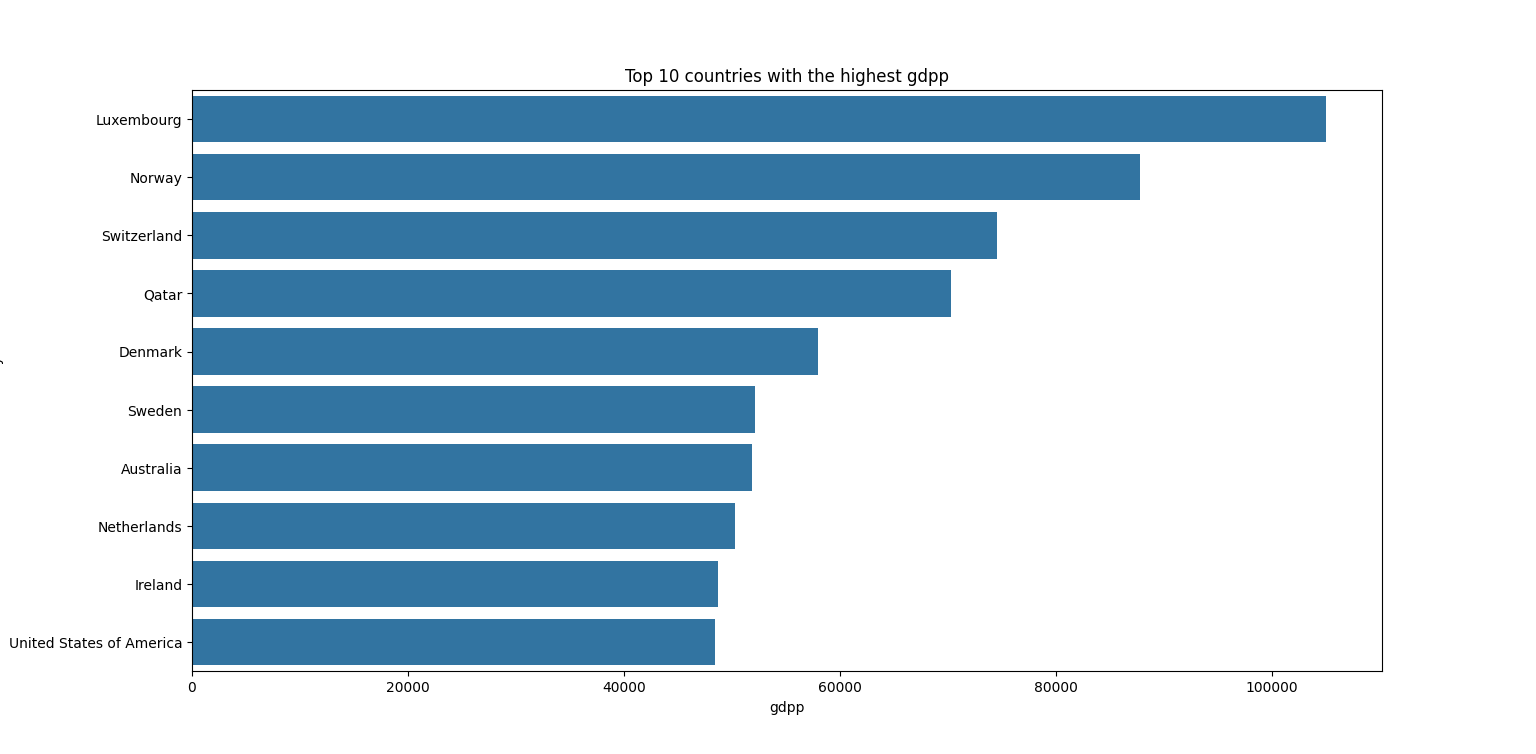
\includegraphics[width=\linewidth]{plot/highest_gdpp.png}
        \caption{Highest GDP per capita}
        \label{fig:highest_gdpp}
    \end{minipage}
    \hfill
    \begin{minipage}{0.8\textwidth}
        \centering
        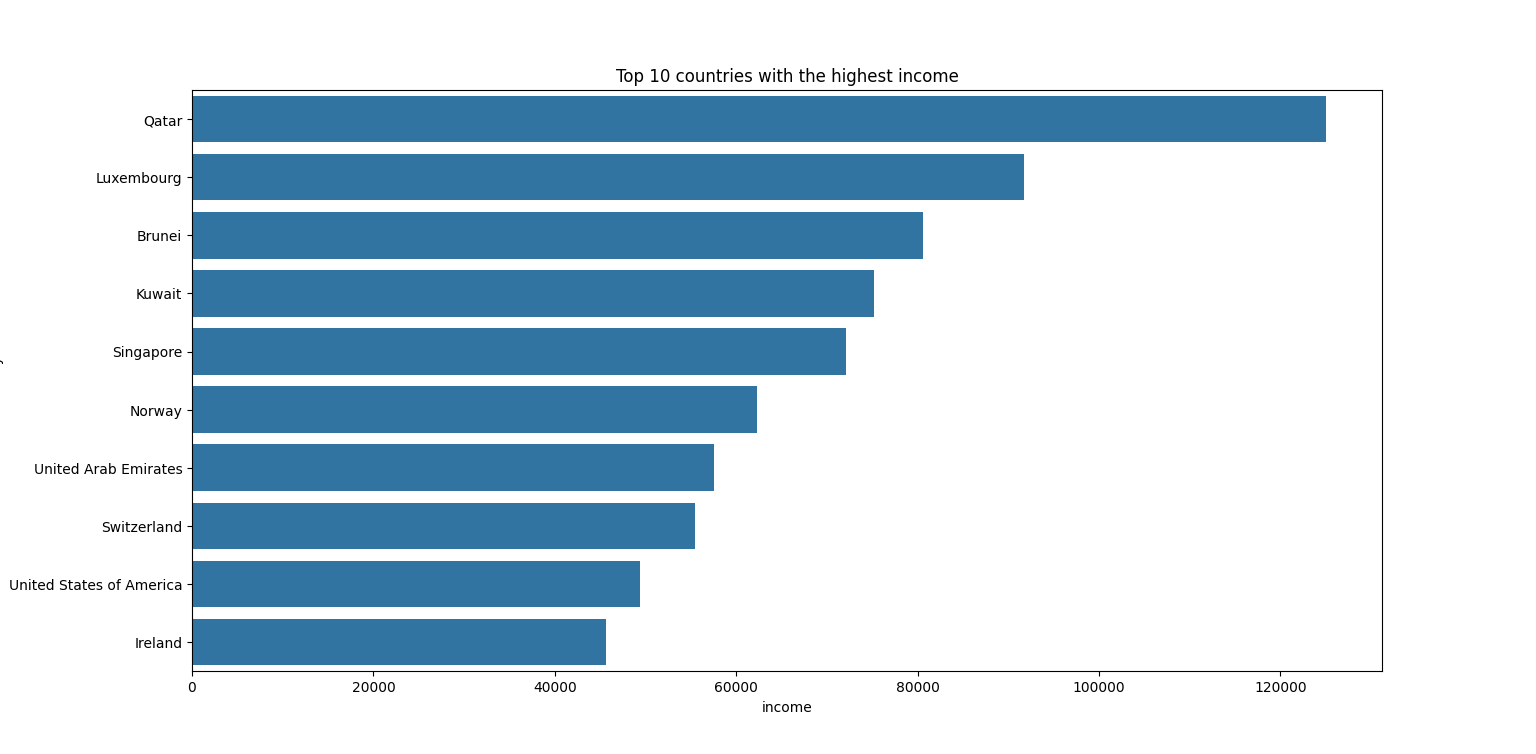
\includegraphics[width=\linewidth]{plot/highest_income.png}
        \caption{Highest Income}
        \label{fig:highest_income}
    \end{minipage}

    % Deuxième ligne
    \begin{minipage}{0.8\textwidth}
        \centering
        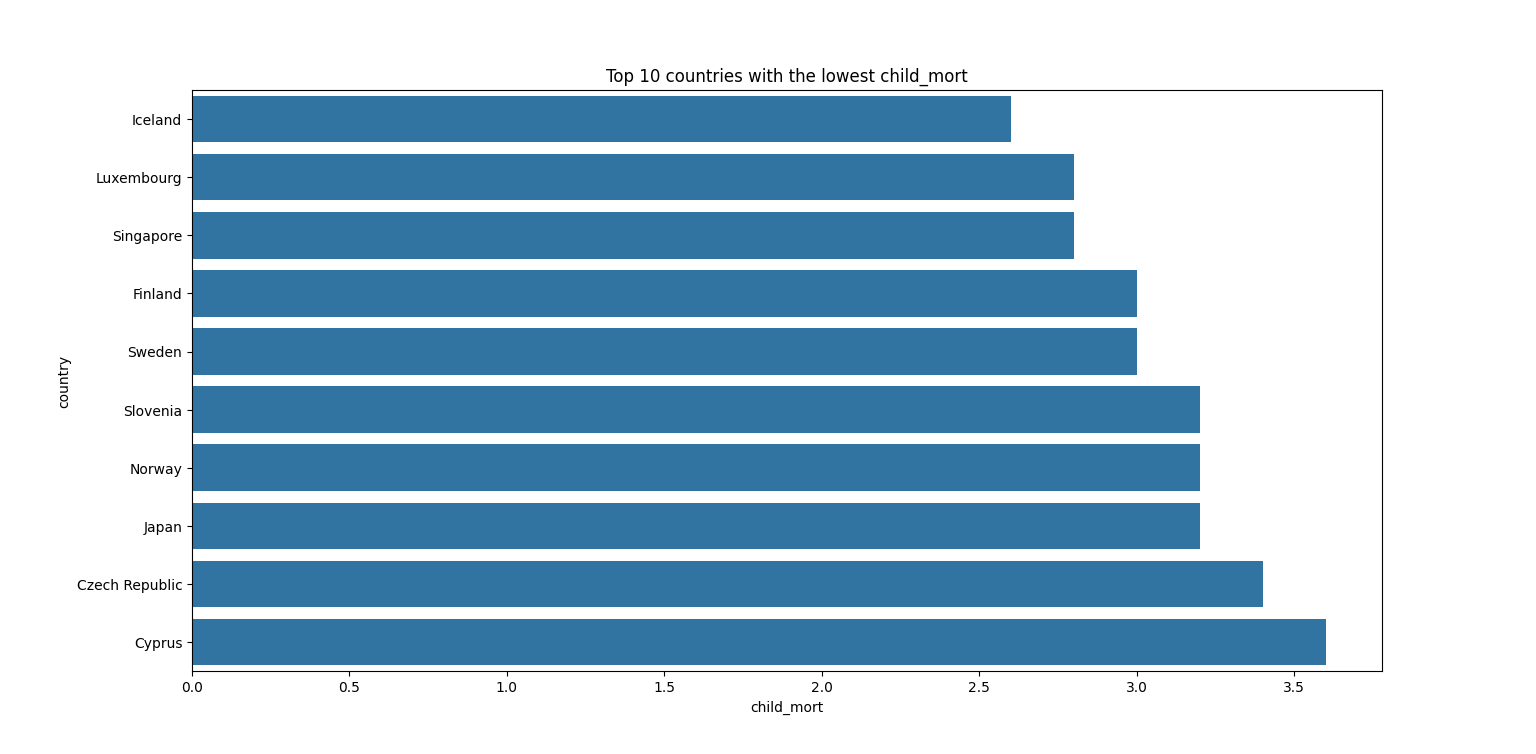
\includegraphics[width=\linewidth]{plot/lowest_child_mort.png}
        \caption{Lowest Child Mortality}
        \label{fig:lowest_child_mort}
    \end{minipage}
    \hfill
\end{figure}

\noindent On peut donc dire que les variables \texttt{gdpp} (\ref{fig:highest_gdpp}), \texttt{income} (\ref{fig:highest_income}) et \texttt{child\_mort} (\ref{fig:lowest_child_mort}) sont très corrélées et peuvent assez bien être représentées par une seule variable. Dans le cadre du TP, nous avons choisi de ne pas éliminer immédiatement les features très corrélées puisqu’elles le seront quand nous ferons la réduction de dimensions (par l’analyse en composantes principales).

\newpage
\section{Pipelining}

\noindent Le modèle de pipeline que nous avons choisi se base sur :

\begin{itemize}
    \item le prétraitement des données.
    \item l’analyse en composantes principales (PCA) pour la réduction de dimension tout en conservant un maximum d'informations. On va passer de 9 dimensions à 2 à 5 dimensions (en fonction du pipeline choisi). Il permet aussi d'éviter les redondances entre les variables corrélées comme avec l'espérance de vie et la mortalité infantile.
    \item les K-means pour le clustering. Il fonctionne très bien avec le PCA et permet d'avoir des clusters bien séparés rapidement.
\end{itemize}

Pour ce qui est du traitement des données, nous avons utilisé deux méthodes :

\begin{itemize}
    \item \texttt{StandardScaler}, il transforme les données de manière à ce que chaque variable ait une moyenne de 0 et un écart-type de 1. Il est très utile pour adapter les données dans un modèle basé sur les distances (comme le nôtre) mais il est sensible aux valeurs extrêmes.
    \item \texttt{MinMaxScaler}, il transforme les données pour qu'elles soient comprises entre 0 et 1 (ou une plage définie). Il est bien adapté aux algorithmes sensibles à l'échelle mais il peut être très influencé par les valeurs extrêmes et n'est pas centré en 0.
\end{itemize}

\noindent Afin de déterminer quel pipeline et quels hyperparamètres sont les meilleurs, nous calculons le \textit{silhouette score} de chaque combinaison. \\ \\
Le \textit{silhouette score} est une métrique qui permet d’évaluer la qualité du clustering. Il mesure la ressemblance des données d’un même cluster (cohésion intra-cluster) tout en s’assurant que les clusters sont bien séparés les uns des autres (séparation inter-cluster). Le \textit{silhouette score} est définie entre -1 et 1. Plus le résultat est proche de 1, plus les clusters sont bien définis et séparés. Aux alentours de 0, les clusters sont mal séparés voire se chevauchent. Une valeur négative indique un mauvais clustering (certains points sont dans le mauvais cluster). \\

\noindent Le meilleur résultat est obtenu avec le pipeline suivant :

\begin{itemize}
    \item \textbf{Prétraitement} : \texttt{StandardScaler}
    \item \textbf{Réduction de dimensions} : \texttt{PCA} (avec 2 composantes principales)
    \item \textbf{Clustering} : \texttt{K-means} (avec 3 clusters)
\end{itemize}

\newpage
\section{Visualisations et analyse des résultats}

\noindent Une fois le pipeline établi, chaque pays obtient une classe (0, 1 ou 2) grâce au K-means à 3 clusters. On peut afficher les différents points en fonctions des deux composantes de l’ACP (en affichant leur cluster comme couleur) :

\begin{figure}[H]
    \centering
    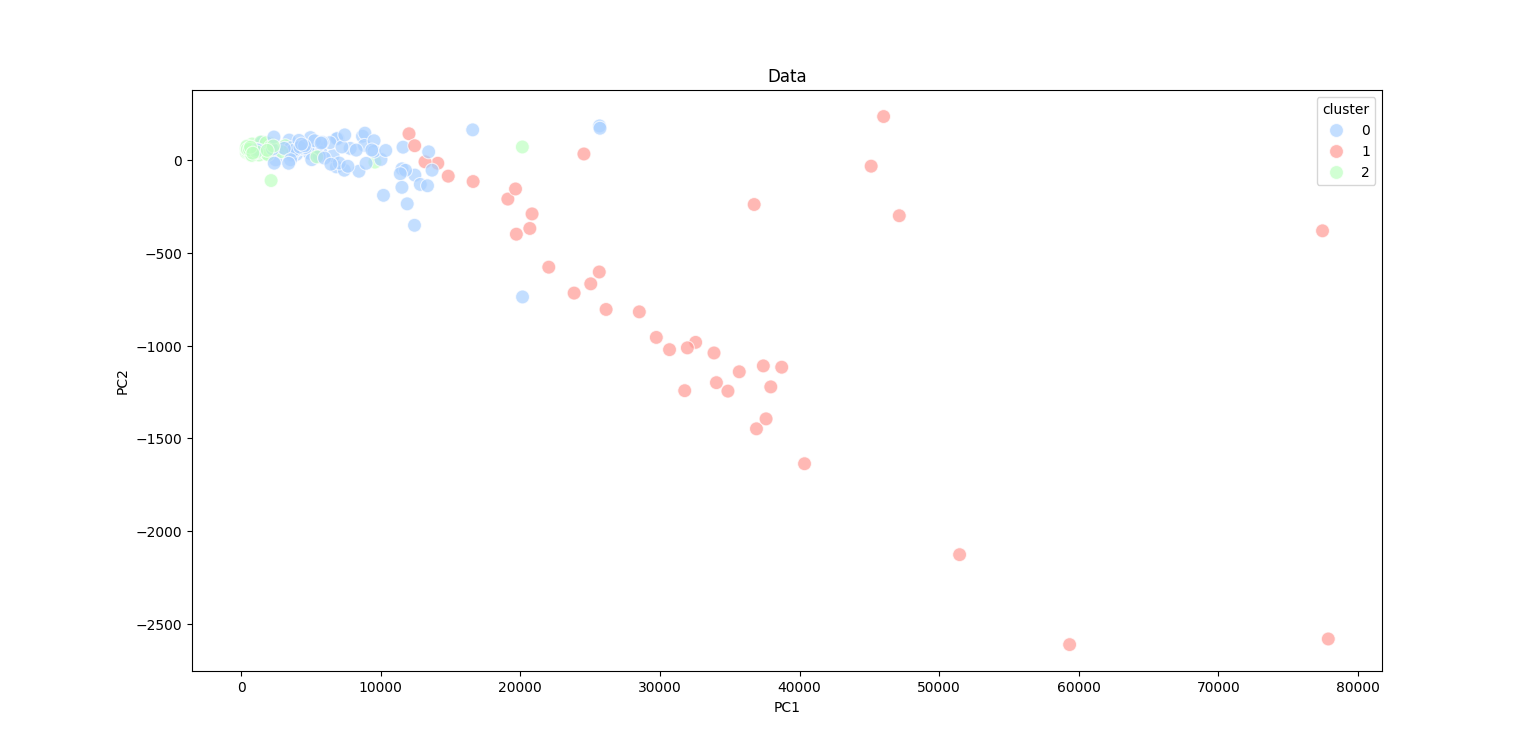
\includegraphics[width=\linewidth]{plot/clusters_pca.png}
    \caption{Clusters PCA}
    \label{fig:clusters_pca}
\end{figure}

\noindent On voit ici (\ref{fig:clusters_pca} de quelle manière ont été regroupés les pays, avec deux groupes très compacts (en vert et en bleu) et un groupe beaucoup plus dispersé (en rouge). \\ \\
Il est ensuite possible de calculer la valeur moyenne de chaque feature pour chacun des trois clusters, on peut donc les comparer.

\begin{figure}[H]
    \centering
    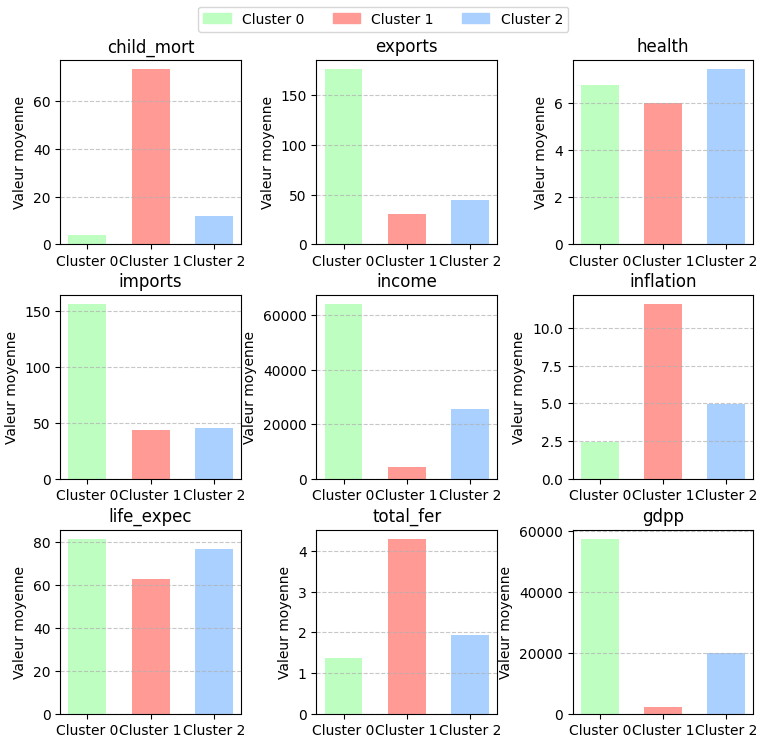
\includegraphics[width=\linewidth]{plot/clusters_features.png}
    \caption{Clusters Features}
    \label{fig:clusters_features}
\end{figure}

\noindent Sur les graphiques ci-dessus (\ref{fig:clusters_features}), on voit que le cluster rouge correspond aux pays qui ont besoin d’aide humanitaire (forte mortalité infantile, faible espérance de vie, forte inflation, faibles revenus…). Au contraire, le cluster vert représente les pays n’ayant pas du tout besoin d’aide (forts imports/exports, PIB par habitant élevé, faible mortalité…). Le cluster bleu se situe plus ou moins entre les deux pour la plupart des features (même s’ils sont largement en dessous du cluster vert pour plusieurs features). \\ \\
Finalement, il est possible de mettre en forme ces données sur une carte du monde (\ref{fig:clusters_map}). Grâce à la librairie python \texttt{geopandas} et au clustering, il est possible de colorier chaque pays en fonction de la classe qui lui a été attribuée par l’algorithme.

\begin{figure}[H]
    \centering
    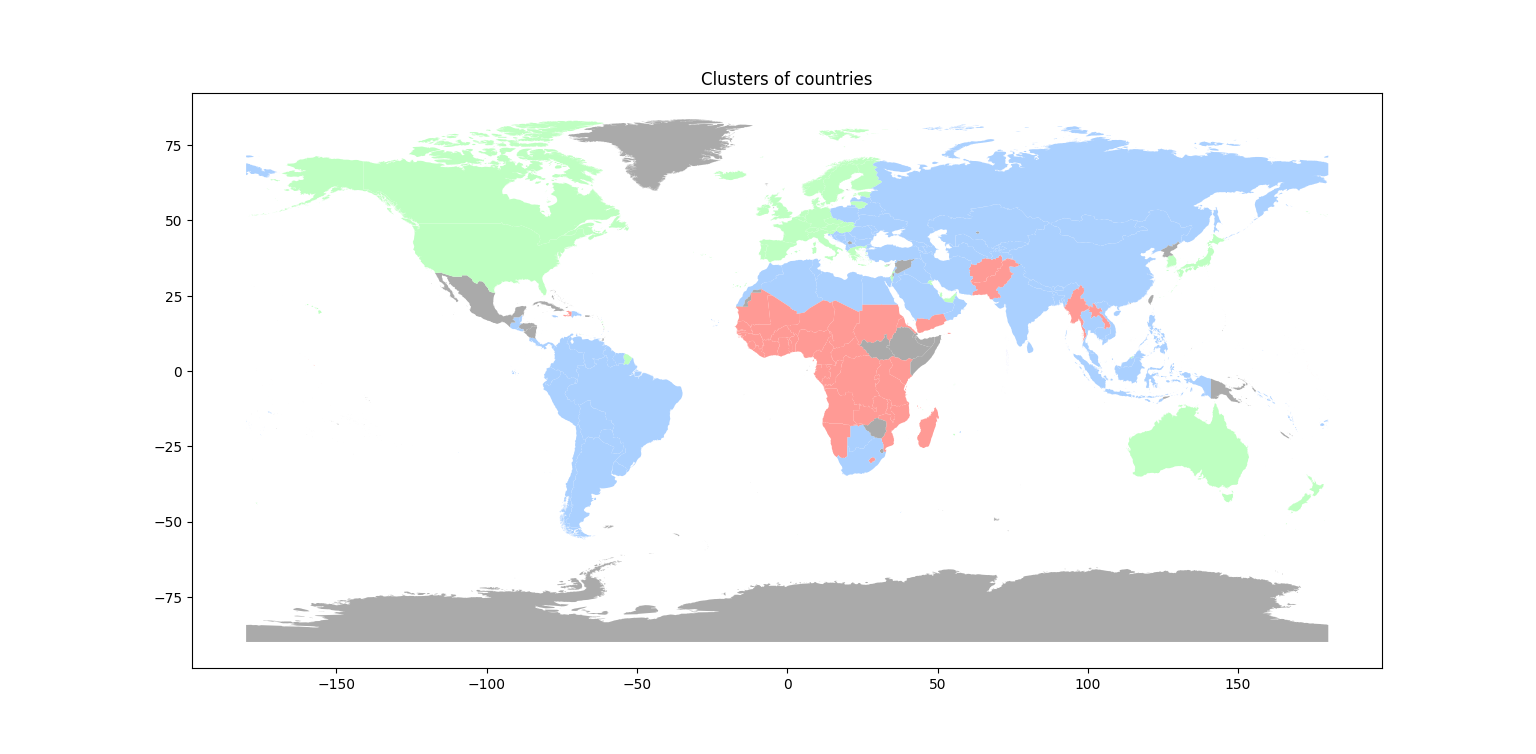
\includegraphics[width=\linewidth]{plot/clusters_map.png}
    \caption{Clusters Map}
    \label{fig:clusters_map}
\end{figure}

\noindent On remarque donc immédiatement que les pays “du Nord” sont généralement en vert, alors que les pays en voie de développement sont plutôt en rouge (surtout en Afrique subsaharienne et en Asie du Sud (Yémen, Pakistan, Afghanistan, Myanmar et Laos)). Cette visualisation a l’air fiable, en effet les pays en rouge sont effectivement ceux qui ont le plus besoin d’aide aujourd’hui. Nous avons testé plusieurs exécutions différentes et à chaque fois, le résultat change légèrement mais reste globalement le même (sauf quelques rares exceptions où le Luxembourg est le seul en vert T-T).

\newpage
\section{L'utilisation de l'IA}

\noindent Nous avons utilisé l'IA (ici ChatGpt et Le Chat de MistralAI) afin de nous aider dans ce projet. Elle a été utilisé dans 3 situations : \\
\begin{itemize}
    \item \textbf{Correction de bug} : lorsque que nous ne trouvions vraiment pas l'erreur, nous lui passons la fonction ainsi que le message d'erreur
    \begin{tcolorbox}[colback=gray!10, colframe=black, title=Prompt (dans Le Chat)]
        (...extrait de code...) \\
        A quoi est due l'erreur suivante : \\
        \texttt{ValueError: n\_components=2 must be between 0 and min(n\_samples, n\_features)=1 with svd\_solver='covariance\_eigh'}
    \end{tcolorbox}
    \item \textbf{Choix des hyperparamètres} : Nous étions un peu perdus quand à la marche à suivre pour cela, nous avons donc utilisé le prompt suivant pour nous orienter dans la bonne direction 
    \begin{tcolorbox}[colback=gray!10, colframe=black, title=Prompt]
Je fais du machine learning sur les données de pays. Je dois faire des pipelines (en python) avec des hyperparamètres différents et choisir un résultat selon un critère qu'il faut définir
Pour l'instant, j'ai cette pipeline :
\end{tcolorbox}
    \item \textbf{LaTeX} : Comme c'est la première fois que nous faisons du LaTeX, nous ne connaisons pas du tout la syntaxe ou les astuces pour faire des flèches ou mettre en avant une partie de texte par exemple.
        \begin{tcolorbox}[colback=gray!10, colframe=black, title=Prompt]
Comment mettre un prompt en latex pour qu'il soit différent du texte 
\end{tcolorbox}
\end{itemize} 

\vspace{1cm}
\noindent Dans ce projet, l'IA nous a permis de mieux appréhender la partie du choix des algorithmes et des hyperparamètres utilisés dans le pipeline. C'est une partie essentielle afin de vérifier que son modèle est cohérent et de l'améliorer. Nous avons aussi pu apprendre plus facilement le LaTeX, les tutoriels que nous avons trouvé en cherchant sur internet n'étaient pas si facilement compréhensibles : ils sont très (trop) complet et on se perd facilement dans les dizaines de pages (et avec l'IA on a pu poser quelques questions personalisées).

\newpage
\section{Conclusion}

\noindent Le modèle de clustering que nous avons mis en place semble être assez fiable pour déterminer les pays qui ont besoin d’aide humanitaire. Il est possible de l’améliorer en faisant un meilleur traitement des données, en ajoutant des données provenant d'autres datasets et en corrigeant les données manquantes. \\ \\
Au cours de ce TP, nous avons appris à manipuler la bibliothèque scikit-learn sur python (qui est super complète pour faire simplement des opérations qui seraient beaucoup plus longues sans), à utiliser des pipelines pour automatiser les traitements et à visualiser des données sur une carte du monde. L'utilisation de données réelles est très intéressante et nous a permis de voir comment des algorithmes de machine learning non-supervisés peuvent être utilisés pour résoudre des problèmes concrets.
\\ \\
Nous avons aussi pu utiliser LaTeX pour la première fois. Nous trouvons que c'est un langage avec beaucoup de possibilités, ce qui semble être à la fois sa force et sa faiblesse. On peut vraiment faire un rapport construit avec du code, des équations, des matrices ... mais cela le rend difficile à appréhender (surtout pour les débutants). Nous préférons tous les deux le rendu de rapport en markdown, HTML ou même Word plutôt qu'en LaTeX, cela peut potentiellement venir du fait qu'on utilise pas très bien le langage :)

\end{document}
